\chapter{Introduction}\label{ch:introduction}
\graphicspath{{../Figures/10-introduction/}{figs/10-introduction/}}

\section{Motivation}

This research pursues two reciprocal goals. The first is to use principles from biomechanics and neuroscience to improve robot autonomy, balance, and adaptability in unstructured terrain \citep{frey_legged_2026, ha_learning_2025, ijspeert_amphibious_2020}. The potential for compliant actuation and neural control to improve locomotor energy economy is a further motivation for this approach.

The second goal is to use robots as controllable physical models of biological movement. Musculoskeletal humanoids and limb systems provide ways to investigate motion generation, internal forces, and neural control hypotheses \citep{asano_design_2017, hitzmann_anthropomorphic_2018}. Robotic models permit repeatable changes to individual actuators or sensory pathways, including interventions that would be impractical or unethical in human participants. They complement animal studies and numerical models by allowing the mechanical and neural contributions to be manipulated together \citep{shin_constructive_2018, goldsmith_investigating_2021}. Work with a salamander robot demonstrates this exchange: biological evidence informed a spinal-cord model, and robotic tests generated predictions that were examined in biological preparations \citep{ijspeert_swimming_2007}. These goals form an iterative cycle: biological knowledge guides more biomimetic robots, robotic experiments generate biological questions, and the resulting understanding can guide further improvements in biomimicry. Prosthetic and orthotic devices are potential applications of this synthesis.

Bioinspired robotics draws broadly on biological principles; biomimetic robots reproduce selected biological structures or mechanisms. Musculoskeletal humanoid robots are a subset of biomimetic robots, using human-like skeletal arrangements and muscle-like actuation. Artificial muscles are a key enabling technology for this project. Among the available actuation technologies, McKibben-style braided pneumatic actuators (BPAs) combine low mass, high force-to-weight ratio, and intrinsic compliance with a force--length curve that qualitatively resembles that of skeletal muscle \citep{liang_comparative_2020, hunt_modeling_2017}. BPAs have been used in quadrupedal robots \citep{aschenbeck_design_2006, hunt_modeling_2017, scharzenberger_design_2019}, musculoskeletal arms \citep{hitzmann_anthropomorphic_2018, kurumaya_musculoskeletal_2016}, and dexterous manipulation systems \citep{chen_realizing_2019}. However, BPAs also differ from biological muscle in important ways: their maximum tensile force occurs at resting length rather than at an optimal fiber length, their maximum contraction ratio is substantially lower than that of human muscle, and their force output is a highly nonlinear function of internal pressure, contraction, and loading state \citep{hunt_modeling_2017, sarosi_comparative_2017, liang_comparative_2020}. My experience with \qty{10}{\mm} actuators made the design gap concrete: at the short resting lengths used in my leg designs, they delivered less force and contraction than I had anticipated from manufacturer specifications. Existing empirical models describe useful pressure--contraction relationships \citep{sarosi_comparative_2017, martens_modeling_2017, hunt_modeling_2017}, but selecting actuators for this robot required predictions across the resting lengths, pressures, and contractions of the tested Festo BPAs. Reliable force prediction is therefore the first requirement for designing the humanoid's actuated joints.

Actuator force alone, however, does not determine the torque a joint produces. A BPA-actuated robot knee transmits actuator force to the skeleton through mounting brackets, artificial tendons, and paths that wrap over the joint, and each of these elements departs from the rigid-body idealization: brackets and fixtures deflect under load, tendons stretch, and a wrapping actuator loses usable length as the knee flexes. For this robot, the effects of compliance and bending and the usefulness of a common correction across knee configurations had not been established experimentally. Here, musculotendon routes are the combined BPA and artificial-tendon paths through attachment and wrapping points. The earlier robot actuator routes were selected from predicted muscle lengths, moment arms, and torque profiles \citep{bolen_determination_2019}. The placement searches that I developed with Morrow and Hunt early in my doctoral research extended that design approach \citep{morrow_optimization_2020}, but their rigid-body predictions still required experimental validation at the knee. The later work in Chapter~\ref{ch:torque} uses those experiments to improve the prediction model and redesign the musculotendon routes.

Researchers implementing neural control models face two related problems. The first is access to physiological evidence. Sensory-afferent findings are distributed across species, preparations, and experimental protocols, so selecting a feedback pathway requires locating its measured properties and the conditions under which they were observed \citep{van_de_crommert_review_1998, windhorst_muscle_2007, windhorst_spinal_2022}. A second problem arises when a published neural circuit is coupled to a different mechanical model: its behavior depends on the actuator mechanics, sensory signals, support conditions, and numerical implementation as well as on the circuit itself. Published architectures and software supply essential components \citep{rybak_modelling_2006, mccrea_organization_2008, markin_afferent_2010, nourse_sns_2023}, but the behavior of their particular combination must be established.

Transferring a controller to different mechanics can require extensive hand tuning. Stepping in suspension alone does not establish that the coupled model can support locomotion on the ground. Efficient development therefore requires both graphical editing of neural circuits and automated evaluation of their interaction with human biomechanical models and BPA-actuated robot models.

I address these gaps through four connected contributions: BPA force characterization with resting length as a design variable, isometric knee-torque prediction and route design, the Sensory Afferent Database, and neuromechanical modeling tools. Together, they provide a basis for selecting actuators, predicting joint output, selecting sensory pathways, and testing neural controllers in coupled models, including virtual-harness-assisted locomotor evaluations.

\section{The Biomimetic Humanoid Robot Project}\label{sec:project}

This dissertation is part of a long-running effort at Portland State University to build a biomimetic humanoid robot representing the body from the lumbar spine down, actuated by pneumatic artificial muscles and controlled by a synthetic nervous system (SNS). The project connects mechanical design and neural-control development through successive physical prototypes and computational models, enabling controlled tests of how actuator mechanics and sensory feedback contribute to movement.

The present work builds directly on a series of studies by me and my collaborators. In my master's project, the kinematics and dynamics of a biomimetic robot leg were matched against the Gait2392 OpenSim model, musculotendon routes, including attachment and wrapping locations, were determined for the robot legs, and MATLAB software was developed for evaluating muscle lengths, moment arms, and isometric joint torques over the full range of motion \citep{bolen_bipedal_2019, bolen_determination_2019}. Hand tuning the placement of artificial muscles was time consuming. The results of that work showed that simply transplanting human muscle attachment locations onto a BPA-actuated robot does not reproduce human torque profiles. The BPA routing optimization developed during this dissertation addresses this limitation and is introduced in Section~\ref{sec:mesh_opt}. Steele designed and validated the biomimetic four-bar knee linkage with a migrating instantaneous center of rotation used in this robot leg \citep{steele_development_2017, steele_biomimetic_2018, steele_biomimetic_2018-1}. Chapter~\ref{ch:torque} measures the isometric torque produced by BPAs acting on that knee.

\section{Research Objectives}\label{sec:objectives}

This dissertation investigates actuator force and knee torque experimentally, consolidates sensory-afferent evidence in the Sensory Afferent Database \citep{bolen_sensory_2023, bolen_using_2024}, and develops neural-model and simulation interfaces with representative verification checks. The objectives are:

\begin{enumerate}
    \item \textbf{Characterize the isometric force of Festo BPAs} with uninflated diameters of \qtylist{10;20}{\mm} over a wide range of resting lengths, contractions, and pressures; derive improved maximum-force and normalized force--strain--pressure models; and compare them against existing models (Chapter~\ref{ch:muscles}).
    \item \textbf{Validate and improve the prediction of isometric knee torque} produced by BPAs on pinned-joint and biomimetic four-bar knees; identify and model losses caused by constant length offsets, series compliance, and actuator bending; and compare the resulting torque envelopes with human capabilities (Chapter~\ref{ch:torque}).
    \item \textbf{Consolidate the sensory afferent literature into a searchable resource}, the Sensory Afferent Database, by auditing and curating the published record of afferent properties across animal species and their role in motor control, and by evaluating AI-assisted screening of candidate papers for expanding the collection (Chapter~\ref{ch:database}).
\item \textbf{Develop and demonstrate neuromechanical modeling tools} by implementing the Li--Deng walker, Gait2392-based models with alternative neural controllers and artificial-muscle actuation, SNS-Simscape blocks for neural pathways coupled with mechanical modeling, and staged tuning and experiment procedures; verify representative circuit responses, implementation agreement, and neural--mechanical signal exchange (Chapters~\ref{ch:sns} and~\ref{ch:overall}).
\end{enumerate}

\section{Dissertation Organization}\label{sec:organization}

Chapter~\ref{ch:background} introduces the robot, BPA actuation, musculoskeletal design, locomotor control, and the scientific rationale for robotic models. Chapter~\ref{ch:muscles} presents the isometric force characterization and actuator models, adapted from my publication \citep{bolen_2026}. Chapter~\ref{ch:torque} tests the joint-torque predictions, identifies compliance and bending-related corrections, and uses them to redesign actuator routes.

Chapter~\ref{ch:database} presents the Sensory Afferent Database, its curation, and its use limits. Chapter~\ref{ch:sns} begins with attempts to transplant published controllers into a different mechanical model, identifies the development requirements exposed by those attempts, and presents the tools and representative checks built to address them. Chapter~\ref{ch:overall} discusses the contributions together and develops the future work; Chapter~\ref{ch:conclusion} states the conclusions. Figure~\ref{fig:roadmap} summarizes these connections.

Appendices~\ref{app:muscle_calcs}--\ref{app:model_geometry} provide the muscle calculations, neural equations, model geometry, and supporting mechanical results. Appendix~\ref{app:simulation_verification} collects the larger simulation evaluations, and Appendix~\ref{app:sadb_records} provides the database coverage and pathway tables.
\begin{figure}[htbp]
\centering
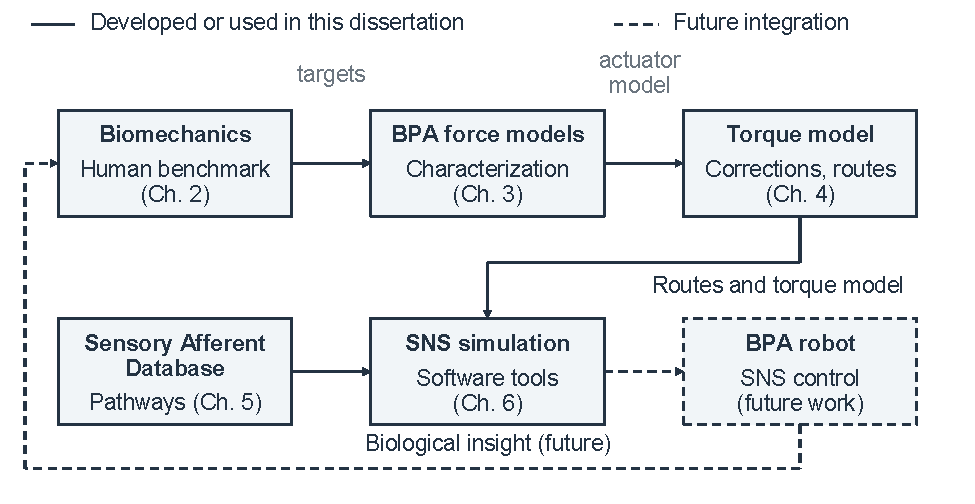
\includegraphics[width=\textwidth]{roadmap.pdf}
\caption[Dissertation roadmap]{Dissertation roadmap. Biomechanical targets guide actuator characterization and route design; the sensory-afferent resource informs feedback selection; and simulation tools support controller evaluation. Dashed connections indicate future integration and the intended return of biological insight.
}
\label{fig:roadmap}
\end{figure}

